\chapter{Appendice A}
\label{appendiceA}
\section{Dataset delle zone sviluppato dal gruppo}
\label{nostraProposta}
Prima di approdare al dataset delle zone di cui abbiamo discusso nella Sez. \ref{zone}, abbiamo ipotizzato e implementato un metodo in grado di restituirci un dataset delle zone in cui suddividere l'Abruzzo prendendo come punto di partenza il dataset delle zone prodotto dall'esecuzione della seguente \textit{query} su PostGreSQL:
\begin{quote}
CREATE TABLE \textit{GeoArea\_split8} (
\newline
\textit{id} serial PRIMARY KEY,
\newline
\textit{geom} geometry (Polygon, 3004))
\newline
\newline
INSERT INTO \textit{GeoArea\_split8} (geom) 
\newline
SELECT ST\_Subdivide(geom,8)
\newline
FROM \textit{Geo\_Area}
\end{quote}

L'invocazione della funzione \textbf{ST\_Subdivide()} sulla geometria che descrive \textit{GeoArea} genera $24142$ zone in cui è suddiviso il territorio abruzzese, di cui è possibile avere una visione d'insieme in Fig. \ref{nostrodataset}.
\begin{figure}[h]
\centering
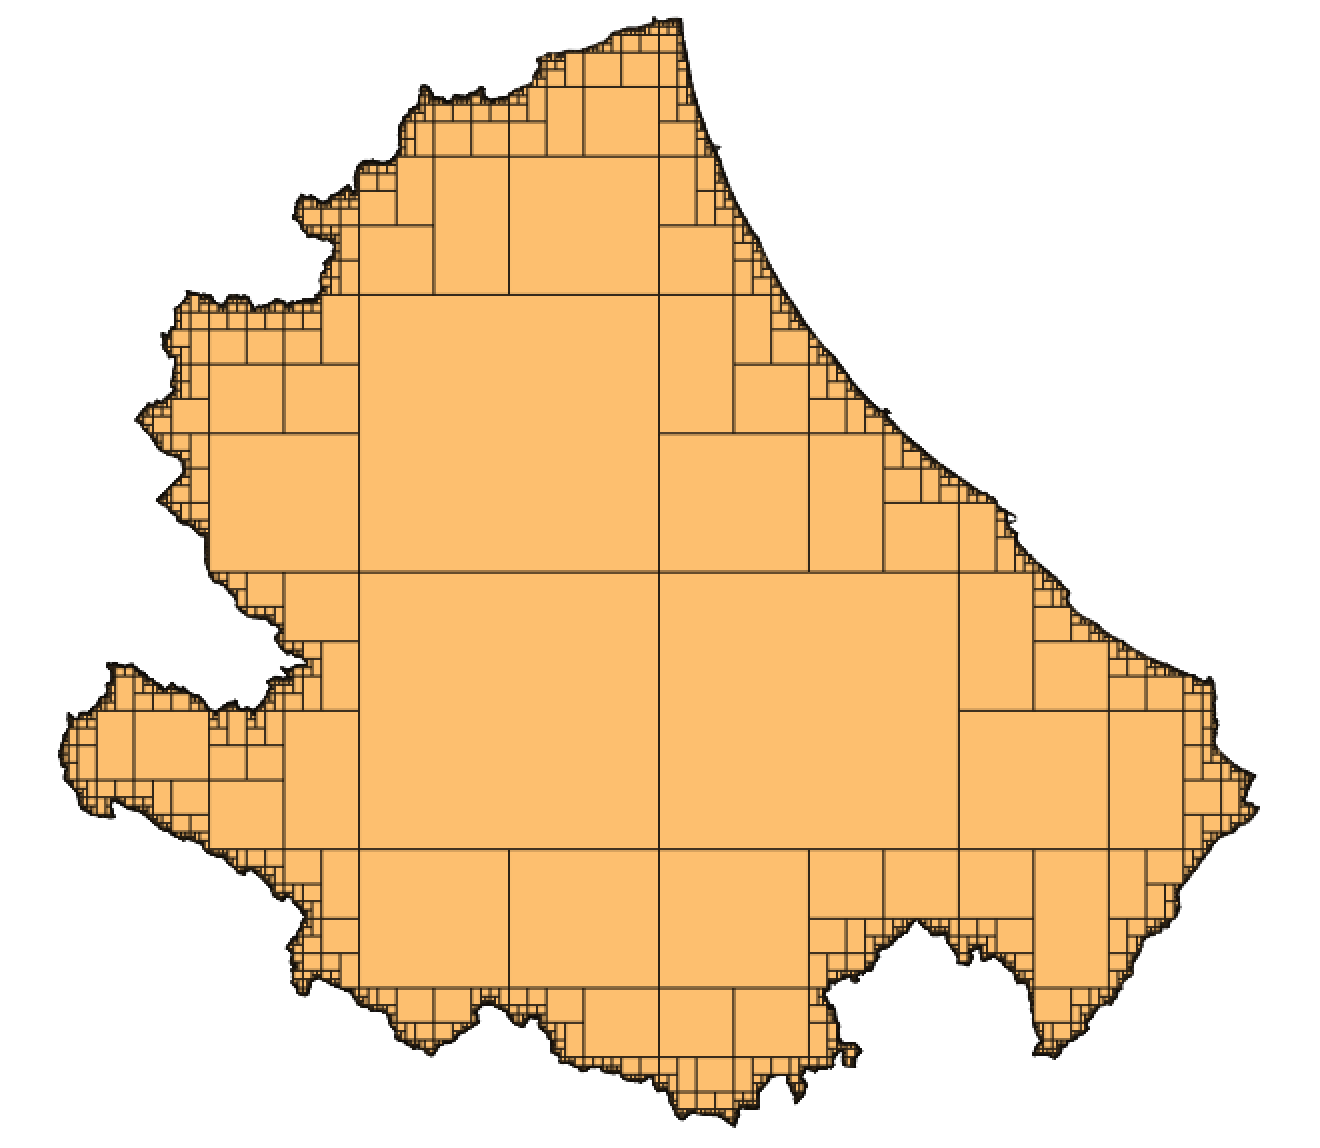
\includegraphics[width=0.4\textwidth]{img/nostrodataset}
\caption{Visione d'insieme delle $24142$ zone generate}
\label{nostrodataset}
\end{figure}
\begin{figure}[h]
\centering
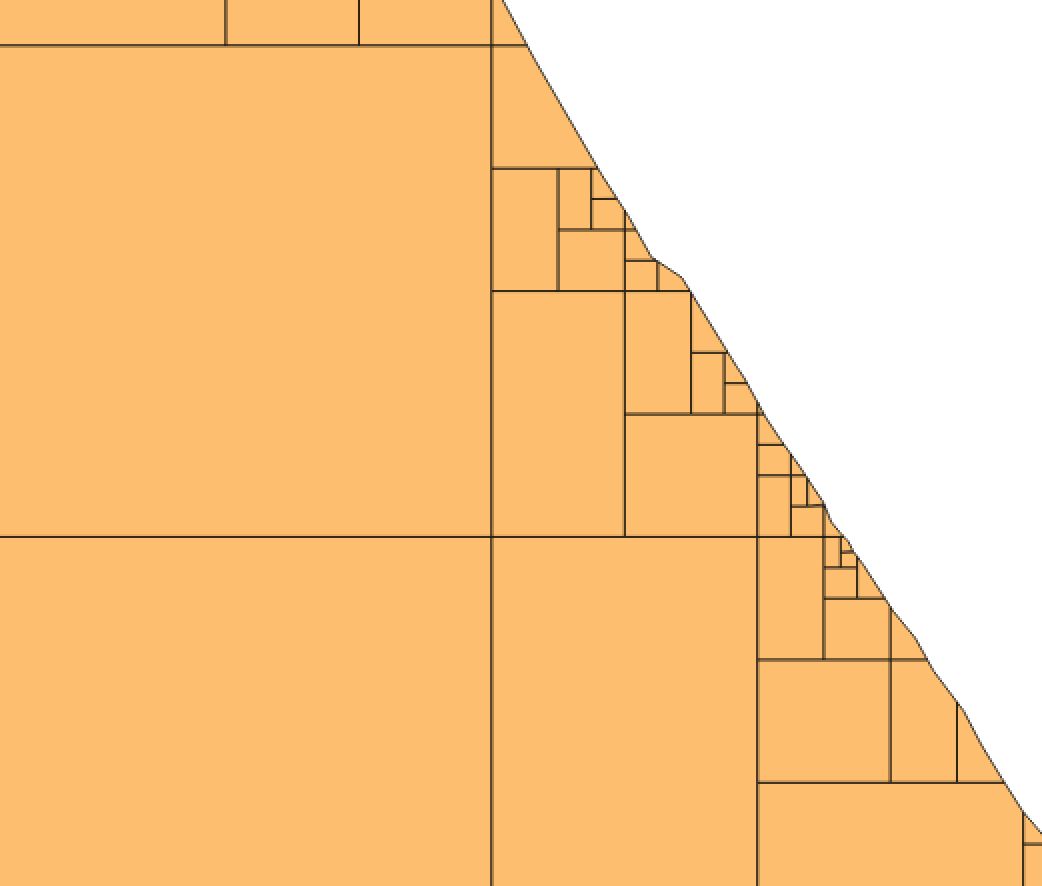
\includegraphics[width=0.3\textwidth]{img/bordo}
\caption{Particolare delle zone in prossimità del \textit{boundary}}
\label{bordo}
\end{figure}
L'esame della Fig. \ref{bordo} fornisce una visione più nitida del tipo di suddivisione effettuata da ST\_Subdivide(). Esso in prossimità del \textit{boundary} della \textit{GeoArea} costruisce poligoni di forma irregolare aventi al massimo otto vertici, mentre tutte le altre aree sono dei quadrati di area crescente via via che ci si sposta verso il centro della \textit{GeoArea}.
Al fine di realizzare un'analisi quantitativa dell'esito del partizionamento della \textit{GeoArea} si riportano in tabella \ref{topMax} e in tabella \ref{topMin} rispettivamente le dieci aree con area maggiore e le dieci con aree minore.

\begin{table}[h]
\centering
\begin{tabular}{|c|c|}
\hline
\rowcolor{lightgray}
Area (kmq)                  & Perimetro (km)             \\
\hline
$3,46$ $\times$ $10^{-11}$  & $3,55$ $\times$ $10^{-5}$  \\
\hline
$1,14$ $\times$ $10^{-10}$  & $5,74$ $\times$ $10^{-5}$  \\
\hline
$3,11$ $\times$ $10^{-10}$  & $8,64$ $\times$ $10^{-5}$  \\
\hline
$3,21$ $\times$ $10^{-10}$  & $8,84$ $\times$ $10^{-5}$  \\
\hline
$6,29$ $\times$ $10^{-10}$  & $19,22$ $\times$ $10^{-5}$ \\
\hline
$6,46$ $\times$ $10^{-10}$  & $14,01$ $\times$ $10^{-5}$ \\
\hline
$6,86$ $\times$ $10^{-10}$  & $14,38$ $\times$ $10^{-5}$ \\
\hline
$8,90$ $\times$ $10^{-10}$  & $16,65$ $\times$ $10^{-5}$ \\
\hline
$11,81$ $\times$ $10^{-10}$ & $19,91$ $\times$ $10^{-5}$ \\
\hline
$13,05$ $\times$ $10^{-10}$ & $17,51$ $\times$ $10^{-5}$ \\
\hline
\end{tabular}
\caption{Top 10 aree più piccole}
\label{topMin}
\end{table}

\begin{table}[h]
\centering
\begin{tabular}{|c|c|}
\hline
\rowcolor{lightgray}
Area (kmq) & Perimetro (km) \\ \hline
$1231,2$   & $140,5$          \\ \hline
$1231,2$   & $140,5$         \\ \hline
$1231,2$   & $140,5$          \\ \hline
$307,8$    & $70,2$           \\ \hline
$307,8$    & $70,2$           \\ \hline
$307,8$    & $70,2$           \\ \hline
$307,8$    & $70,2$           \\ \hline
$307,8$    & $70,2$           \\ \hline
$307,8$    & $70,2$           \\ \hline
$307,8$    & $70,2$          \\ \hline
\end{tabular}
\caption{Top 10 aree più grandi}
\label{topMax}
\end{table}


Come si può vedere chiaramente i valori del perimetro e dell'area delle varie zone presentano davvero molti ordini di grandezza di differenza, ragion per cui è necessario un duplice approccio di elaborazione allo scopo di ottenere un dataset delle zone tale per cui le varie zone abbiano un'estensione quantomeno paragonabile tra loro:
\begin{itemize}
\item Frazionamenti successivi dei poligoni interni "\textit{enormi}" ;
\item Accorpamenti successivi dei poligoni lungo il bordo.
\end{itemize}
\subsection{Processamento dei poligoni interni}
Al fine di realizzare un algoritmo in grado di realizzare dei frazionamenti successivi dei poligoni interni "enormi" presenti nel dataset delle zone che abbiamo preso come punto di partenza abbiamo realizzato uno studio della funzione \textbf{ST\_Subdivide()}, con lo scopo di comprendere quali sono i suoi limiti applicativi. Da questo studio è emerso che tale funzione risulta essere inapplicabile per $1257$ delle $24142$ zone in cui abbiamo diviso il territorio. Questi $1257$ elementi presentano un'area maggiore di $0,1$ kmq e hanno numero di vertici inferiore ad $8$, motivo per cui non sono processabili ulteriormente tramite la funzione ST\_Subdivide().\newline
Abbiamo ricercato dunque un'altra funzione che potesse venirci in aiuto per raggiungere il nostro obiettivo e consultando il manuale PostGIS 2.3.2dev abbiamo ritenuto opportuno utilizzare la funzione \textbf{ST\_Segmentize} per processare queste $1257$ zone "\textit{problematiche}". Applicando tale funzione abbiamo ottenuto $37875$ zone geometricamente omogenee la cui area massima è pari a $0,5$ kmq. E' stato necessario, di conseguenza, implementare un meccanismo di aggregazione di tali zone con lo scopo di ottenere zone geometricamente eterogenee. Il metodo di aggregazione che abbiamo proposto e implementato sfrutta approccio \textit{random}: \newline
Per 1/3 delle zone, scelte in maniera random tra tutte le zone "problematiche", abbiamo utilizzato la funzione \textbf{ST\_buffer()}, con centro situato nel centroide della zona e raggio pari a $400$ m, per individuare le zone confinanti con essa, candidate ad essere aggregate; Tra tutte le zone candidate ad essere aggregate, individuo in maniera random una di queste e tramite la funzione \textit{ST\_Relate} determino se esse sono effettivamente confinanti. Nel caso in cui la loro intersezione è una linea/geometria di dimensione 1, avviene effettivamente l'aggregazione. Questa operazione di aggregazione avviene un massimo di tre volte.
\subsection{Processamento dei poligoni lungo il bordo}
Come abbiamo già discusso nella Sez. \ref{nostraProposta} le zone presenti sul bordo hanno un'area distante molti ordini di grandezza rispetto l'obiettivo che ci siamo prefissati. Di conseguenza è stato necessario implementare un meccanismo di aggregazione di tali zone con lo scopo di ottenere delle aree con estensione più accettabile e vicina al valore medio che ci siamo posti come obiettivo: \newline
\begin{itemize}
\item Per ogni zona problematica del bordo, che andremo a chiamare $z_{bordo}$, andiamo a realizzare un buffer con un certo raggio (che a livello implementativo abbiamo fissato a $150$m) con lo scopo di costruire un cerchio.
\item Tale cerchio verrà intersecato, tramite la funzione \textbf{ST\_Intersect()}, con tutte le zone problematiche del bordo al fine di individuare quali sono le zone che intersecano la sua geometria, che andremo a chiamare $z_{cerchio}$.
\item Per ogni $z_{cerchio}$, sfruttando la funzione \textbf{ST\_Relate} e la definizione di \textit{DE-9IM matrix pattern}, riusciamo a stabilire se risulta essere adiacente con la zona $z_{bordo}$ (la funzione \textbf{ST\_Relate} restituirà \textit{true} o \textit{false} se l'intersezione tra le due zone, rappresentate come poligoni, è una linea/geometria di dimensione 1).
\item Una volta individuate tutte le zone adiacenti alla zona presa in esame, che indicheremo con $z_{adiacente}$, opero un'operazione di aggregazione ovvero unisco la $z_{bordo}$ con la $z_{adiacente}$ più piccola. Se dall'unione risulta che l'area è ancora troppo piccola ripeto l'operazione di aggregazione.
\end{itemize}
\subsection{Conclusioni}
Le operazioni realizzate sia sul bordo che all’interno per realizzare le aggregazioni, così come le abbiamo pensate ed implementate, risultano essere molto pesanti, anzi quasi infattibili per un numero così elevato di elementi.

\section{QuantumGIS}
Uno strumento software che è risultato indispensabile nello studio metodologico-sperimentale descritto in questo documento è il software QuantumGIS (QGIS) nella versione 2.18.2. Trattasi di un software open source, scritto in C+ e distribuito sotto licenza GNU General Public License, orientato ad agevolare coloro che hanno esigenza di operare su dati geografici/territoriali. La versione che abbiamo utilizzato supporta moltissimi formati raster e vettoriali, supporto che si amplia con l'uso dei plugins esterni, come ad esempio Qgis2threejs e QuickWKT. \newline
Il plugin \textbf{Qgis2threejs} è un visualizzatore 3D basato sulla tecnologia WebGL e sulla libreria Javascript three.js che ci è risultato molto utile nello studio della morfologia del terreno e di conseguenza nella validazione dei risultati ottenuti dai metodi descritti in questo documento. 
Un altro plugin che ci è risultato utile nello studio è \textbf{QuickWKT}, ovvero un plugin in grado di mostrare facilmente i dati WKT / WKB in QGIS. \newline
L'utilità di tale GeoViewer è evidente in quanto i dati vettoriali e raster e le tabelle spaziali utilizzati dalle \textit{query} implementate su PostGreSQL sono difficilmente interpretabili e risulta quindi evidente la necessità di avere un tool in grado di visualizzarli. QGIS utilizza la libreria OGT per leggere e creare vettori (comunemente chiamati \textit{layers}) a partire da ESRI shapefiles o da dati spaziali PostGis. E' possibile creare un layer QGIS a partire da dati spaziali memorizzati in un database PostGreSQL/PostGIS e i vari layer aperti in un certo istante della sessione di lavoro sono elencati nella finestra di QGIS denominata \textit{legenda} e vengono contestualmente sovrapposti nella finestra grande sulla destra nello stesso ordine con il quale sono elencati nella \textit{legenda}. Uno strumento di QGIS che ci è risultato molto utile è "\textit{Informazioni Elementi}", che ci consente di interagire con gli elementi presenti nel layer rappresentato nella finestra grande per conoscerne le proprietà geometriche e descrittive. 
